\chapter{Практическая часть}

На рисунке~\ref{ex:r1} представлены построенные графики по заданным параметрам для равномерного распределения.

\begin{figure}[ht!]
	\centering
	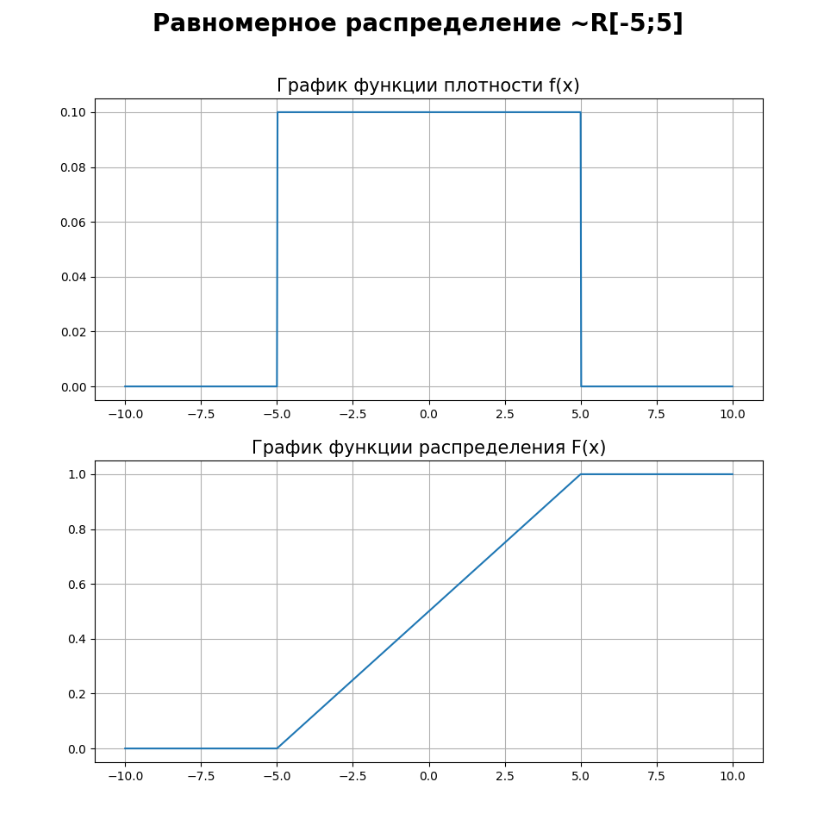
\includegraphics[width=0.8\linewidth]{img/r1.png}
	\caption{Равномерное распределение при a = -5 и b = 5}
	\label{ex:r1}
\end{figure}

\clearpage

%\begin{figure}[ht!]
%	\centering
%	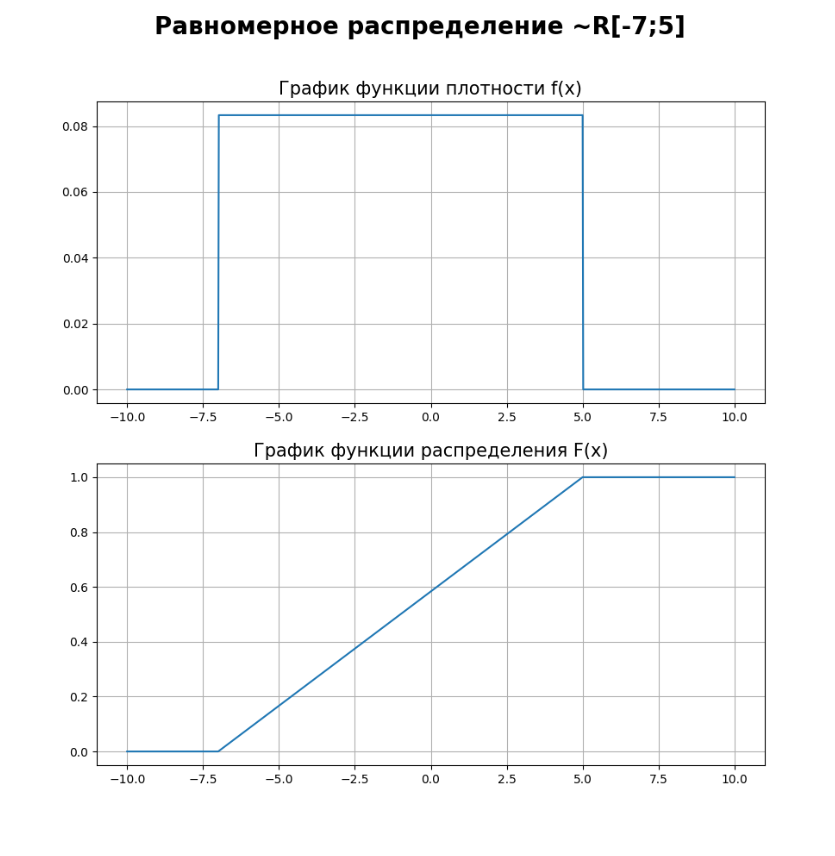
\includegraphics[width=0.8\linewidth]{img/r2.png}
%	\caption{Равномерное распределение при a = -7 и b = 5}
%	\label{ex:r2}
%\end{figure}

%\clearpage
%
На рисунке~\ref{ex:n1} представлены построенные графики по заданным параметрам для нормального распределения.

\begin{figure}[ht!]
	\centering
	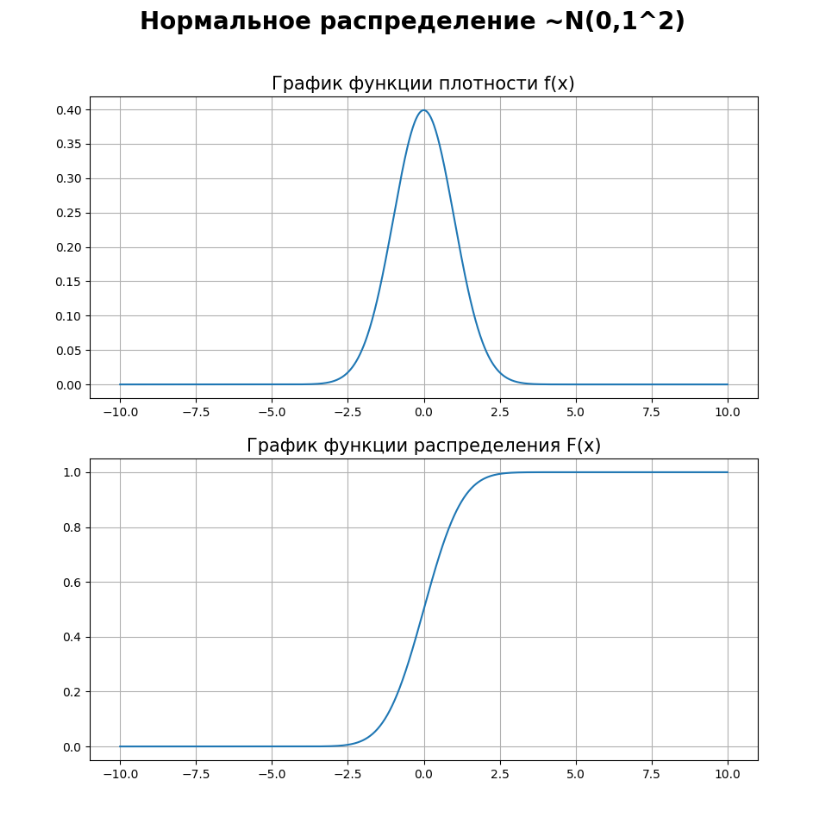
\includegraphics[width=0.8\linewidth]{img/n1.png}
	\caption{Нормальное распределение при m = 0 и $\sigma$ = 1}
	\label{ex:n1}
\end{figure}

\clearpage
%
%\begin{figure}[ht!]
%	\centering
%	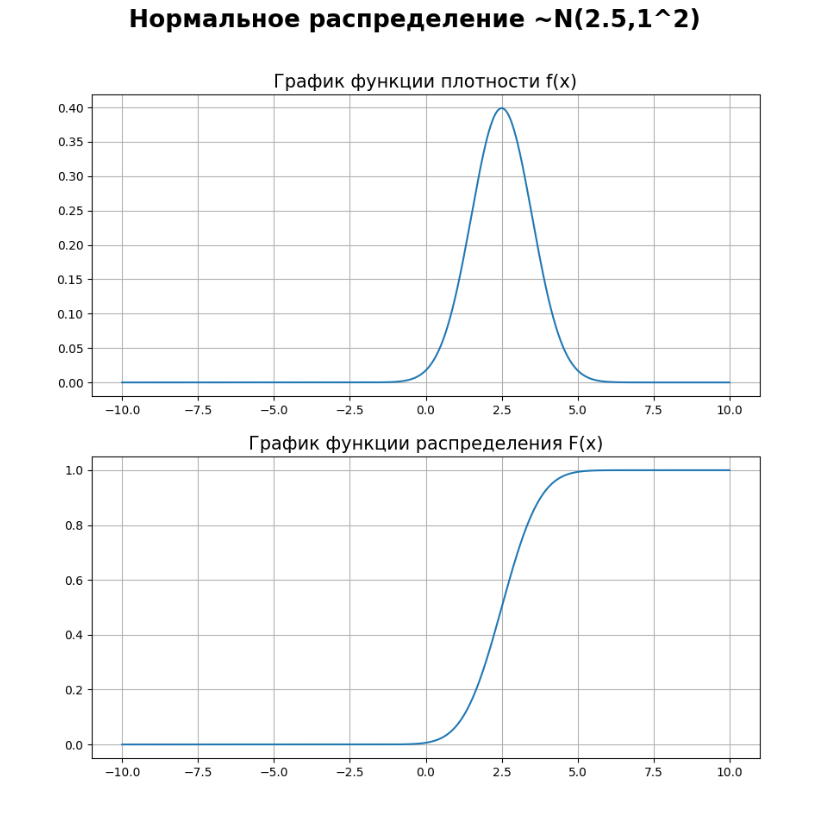
\includegraphics[width=0.8\linewidth]{img/n2.png}
%	\caption{Нормальное распределение при m = 2.5 и $\sigma$ = 1}
%	\label{ex:n2}
%\end{figure}
%
%\clearpage
%
%\begin{figure}[ht!]
%	\centering
%	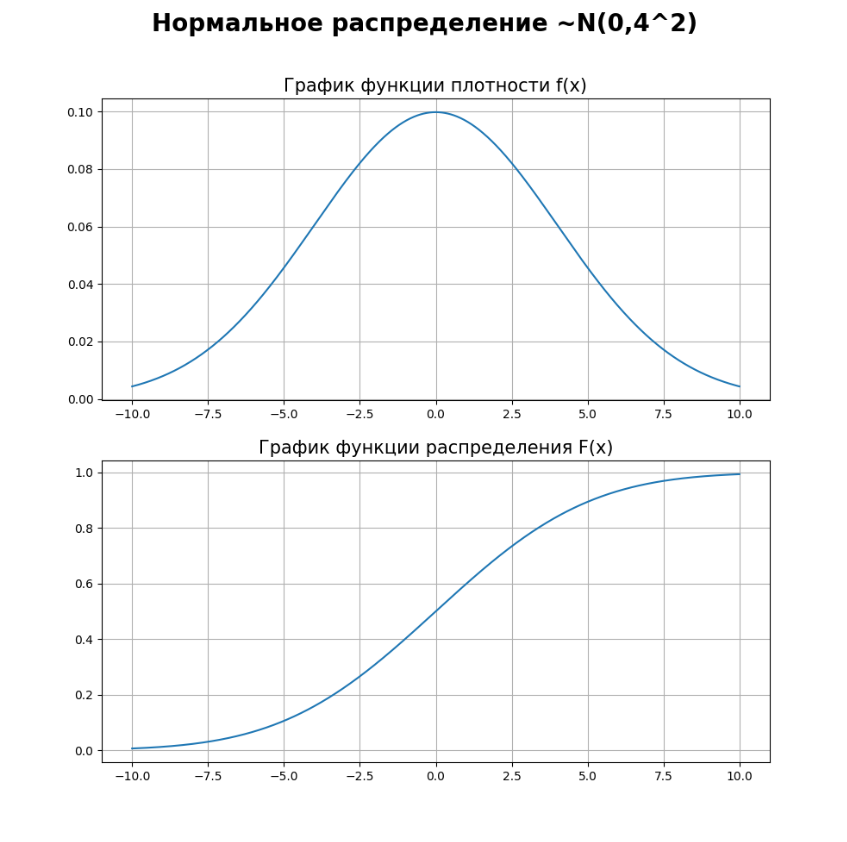
\includegraphics[width=0.8\linewidth]{img/n3.png}
%	\caption{Нормальное распределение при m = 0 и $\sigma$ = 4}
%	\label{ex:n3}
%\end{figure}